\subsection{Energetics Results}
\label{subsection:energeticsresults}

Figure \ref{fig:energy_gamma_n} shows the normalised energy cost on the two neutral surfaces considered in the previous sections. Though the variance on the surface is small there are some areas where the energy cost is non-zero and even negative. The negative energy cost appears to be approximately 10 times smaller in magnitude than the positive energy cost.

\begin{figure}[htbp]
    \centering
     \begin{subfigure}[b]{0.4\textwidth}
         
         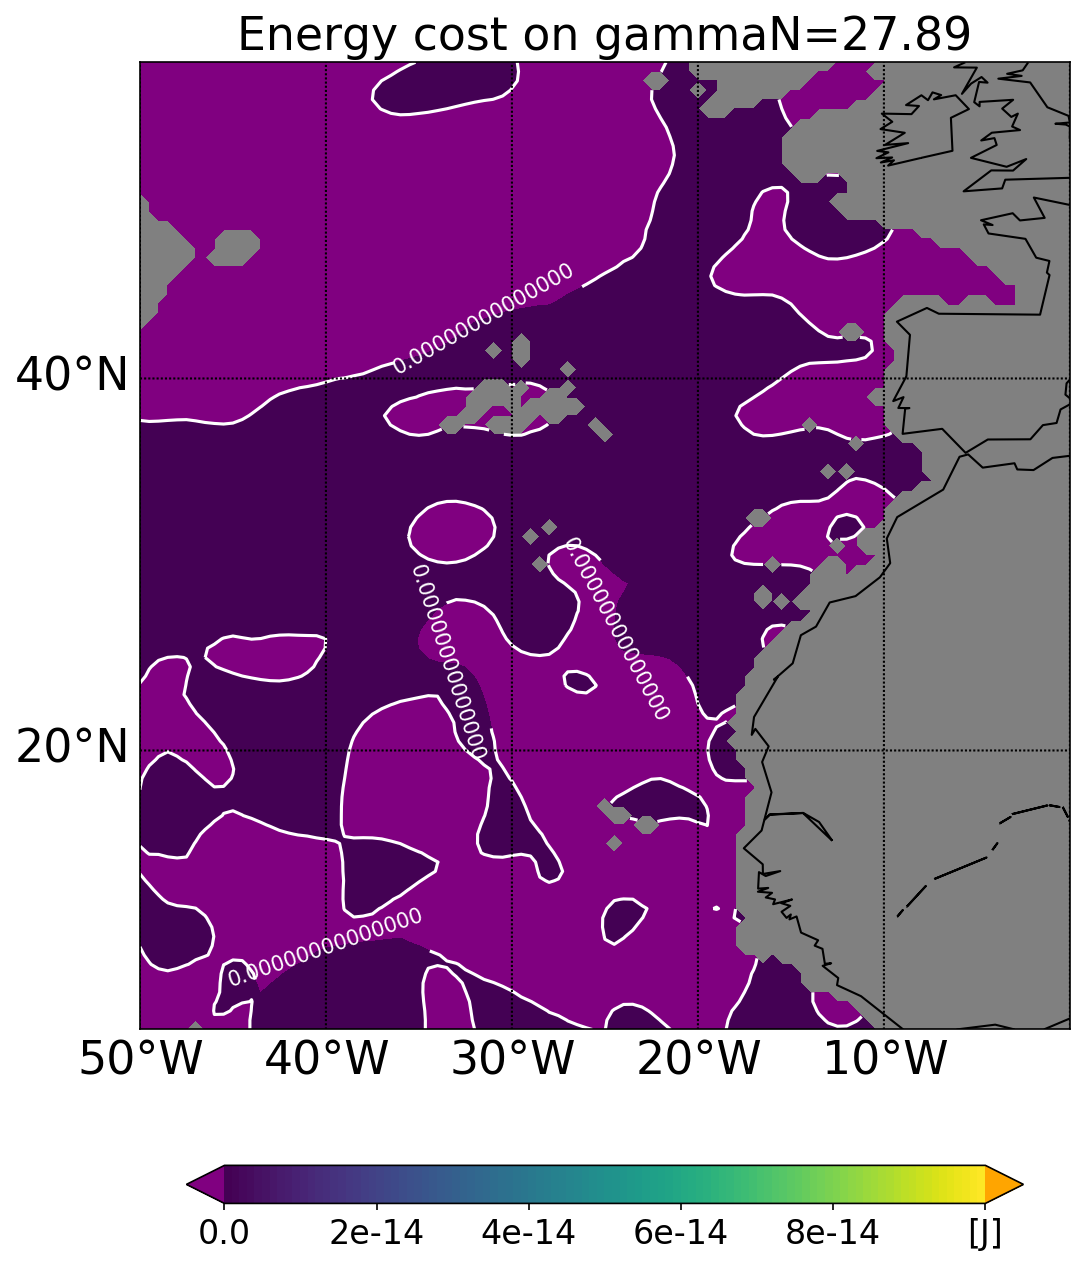
\includegraphics[width=\textwidth]{plots/energy/atlantic_energy/Map2dcyl_energy_on_gammaN_2789e-2_reg310Eto360E05Nto57N_1990to1998av_WOCE.png}
         \caption{$\frac{\Delta E}{d^2}$ on $\gamma_n = 27.89$, Atlantic}
         \label{fig:subplot_atlantic_energy_gamma_n}
     \end{subfigure}
     \hfill
     \begin{subfigure}[b]{0.4\textwidth}
         
         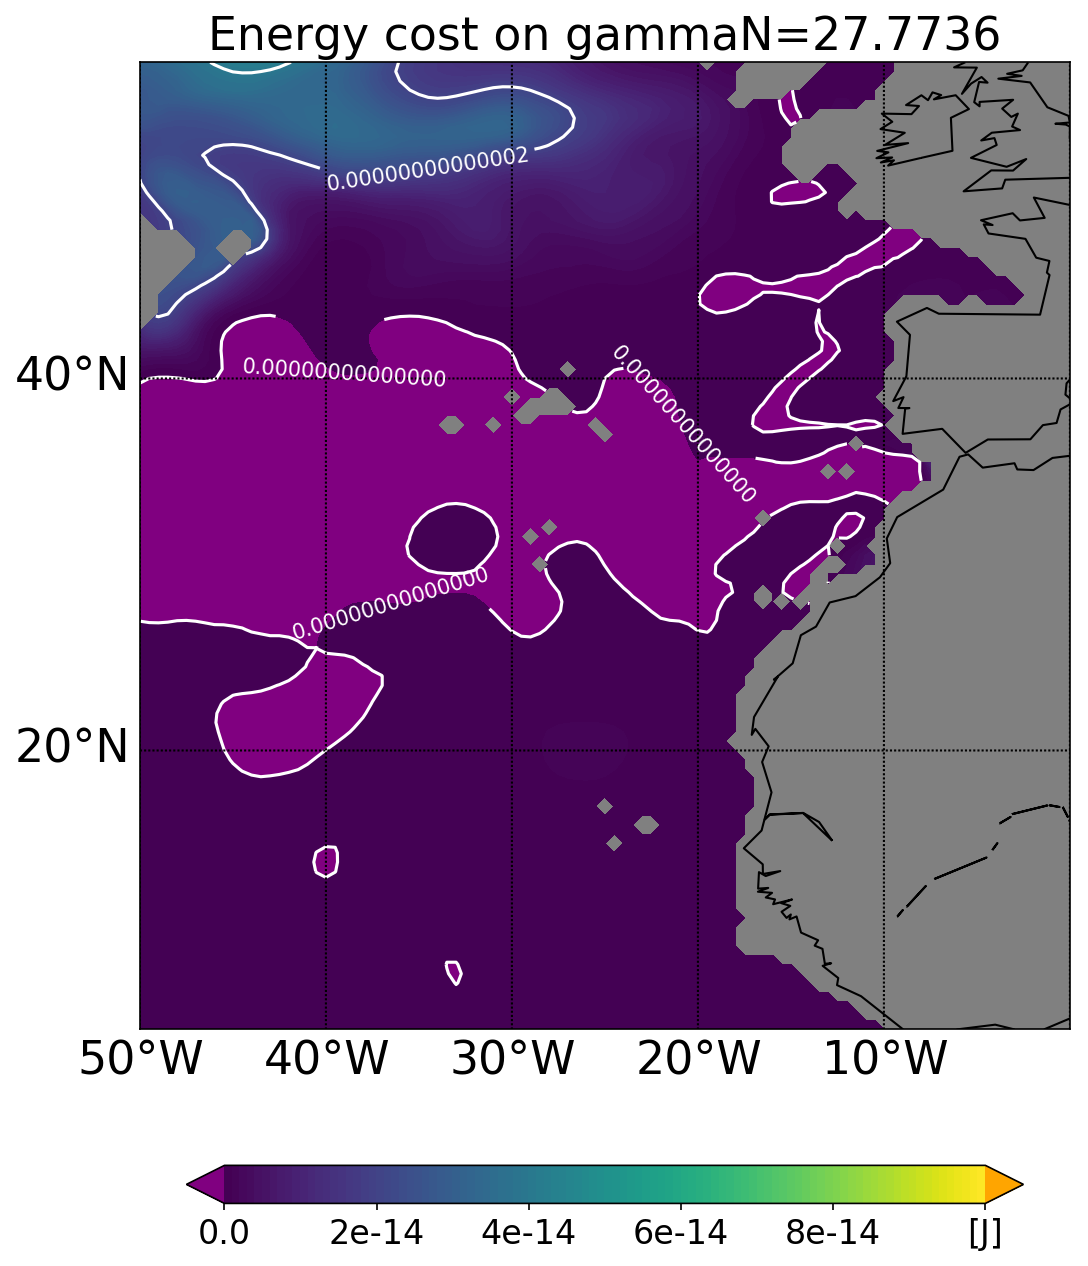
\includegraphics[width=\textwidth]{plots/energy/gibraltar_energy/Map2dcyl_energy_on_gammaN_2777e-2_reg310Eto360E05Nto57N_1990to1998av_WOCE.png}
         \caption{$\frac{\Delta E}{d^2}$ on $\gamma_n = 27.7736$, Gibraltar}
         \label{fig:subplot_gibraltar_energy_gamma_n}
     \end{subfigure}
     \hfill
      \begin{subfigure}[b]{0.4\textwidth}
         
         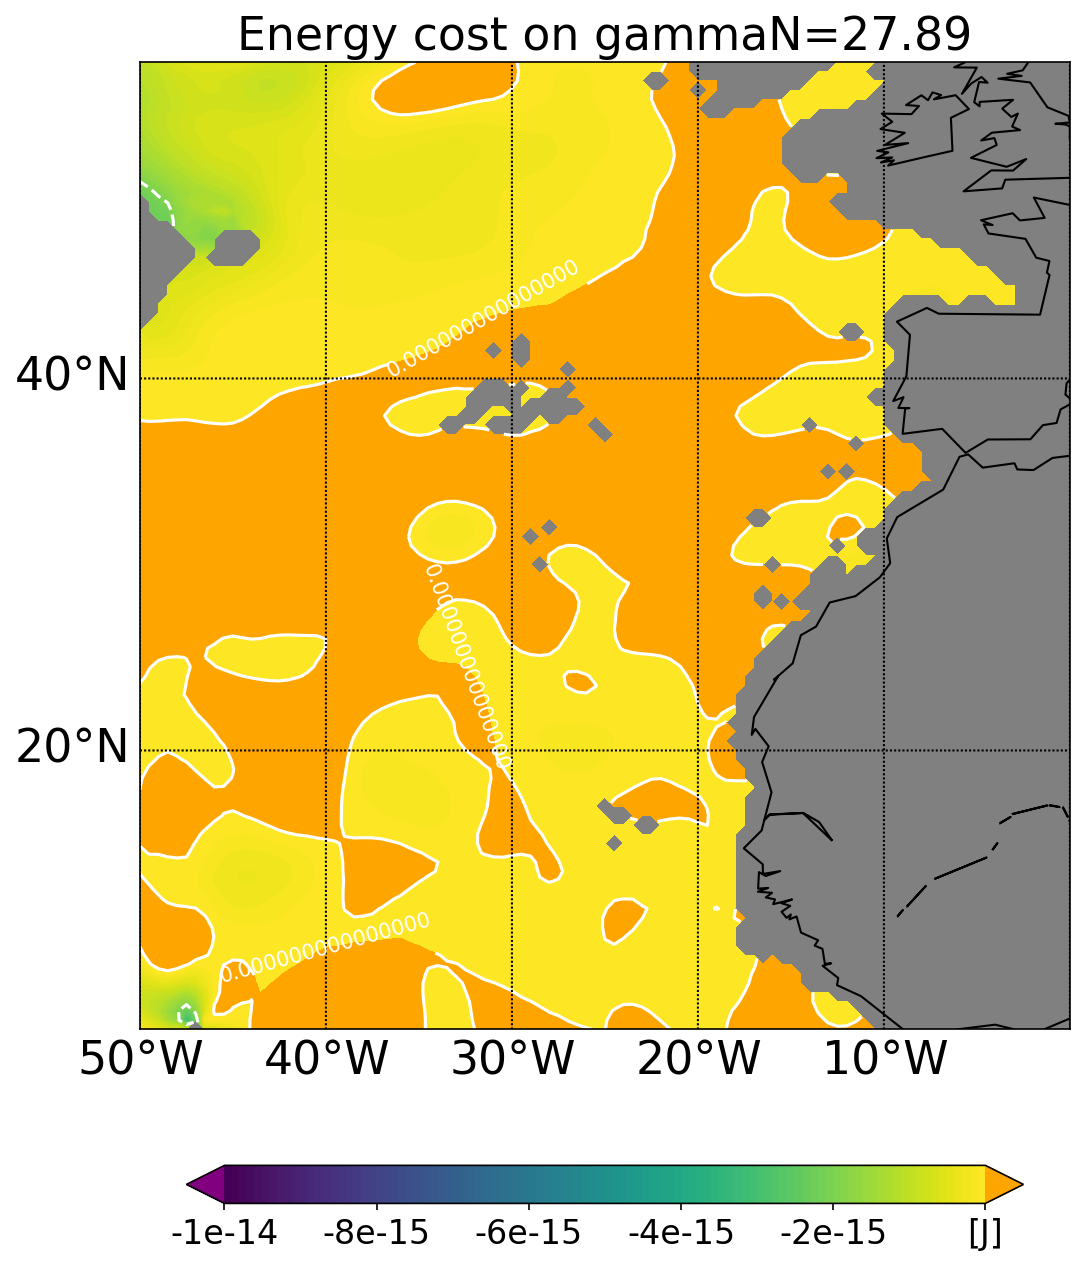
\includegraphics[width=\textwidth]{plots/energy/atlantic_energy/Map2dcyl_neg_energy_on_gammaN_2789e-2_reg310Eto360E05Nto57N_1990to1998av_WOCE.png}
         \caption{$\frac{\Delta E}{d^2}$ on $\gamma_n = 27.89$, Atlantic}
         \label{fig:subplot_atlantic_neg_energy_gamma_n}
     \end{subfigure}
     \hfill
     \begin{subfigure}[b]{0.4\textwidth}
         
         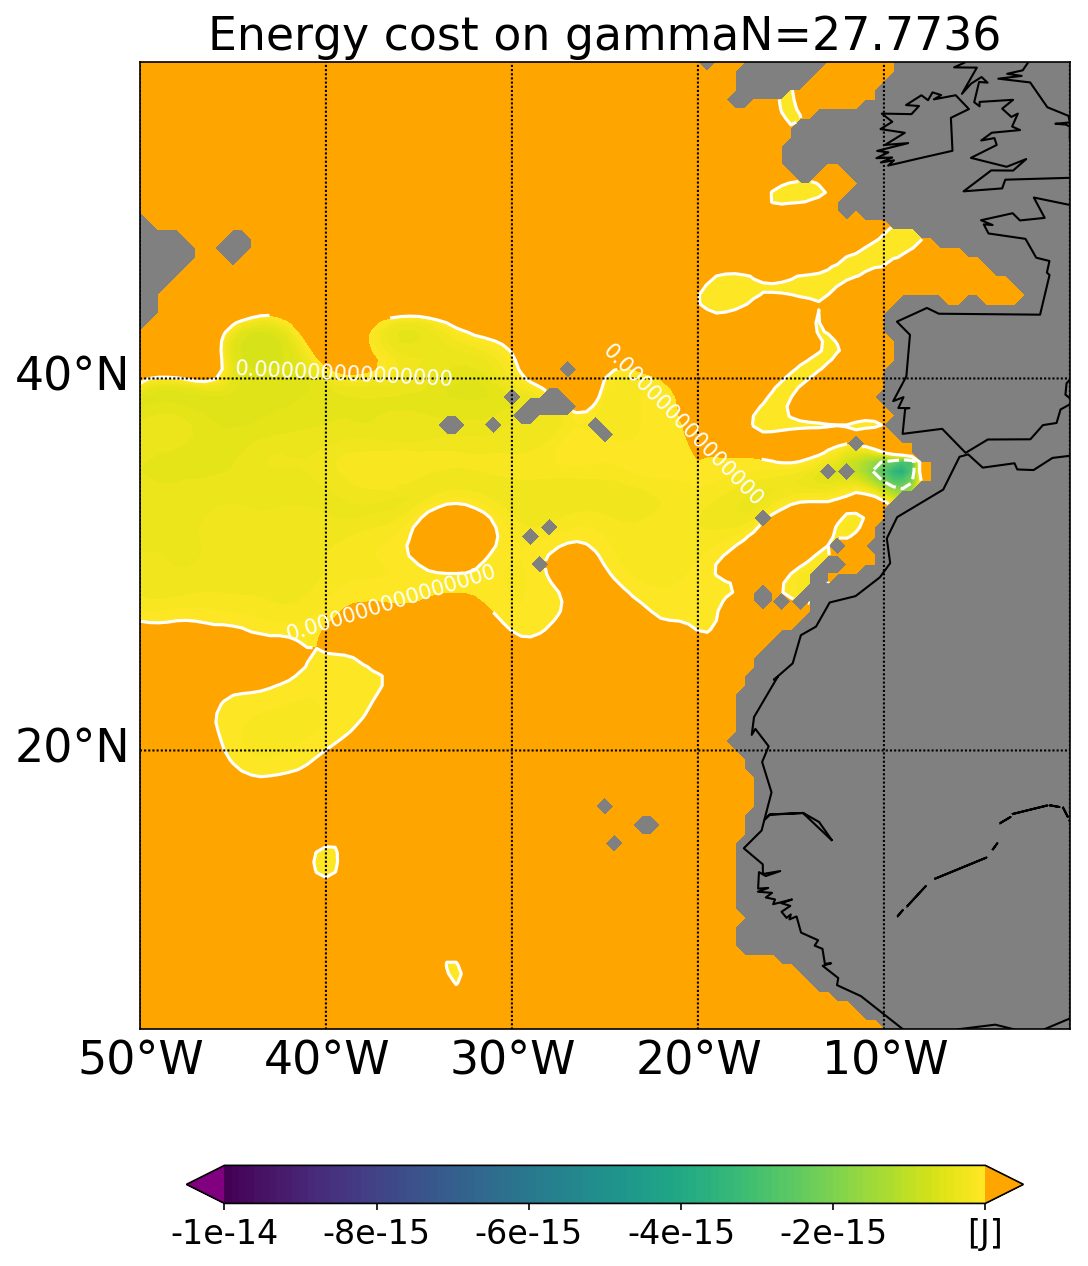
\includegraphics[width=\textwidth]{plots/energy/gibraltar_energy/Map2dcyl_neg_energy_on_gammaN_2777e-2_reg310Eto360E05Nto57N_1990to1998av_WOCE.png}
         \caption{$\frac{\Delta E}{d^2}$ on $\gamma_n = 27.7736$, Gibraltar}
         \label{fig:subplot_gibraltar_neg_energy_gamma_n}
     \end{subfigure}
     
    \caption{The normalised energy cost, $\frac{\Delta E}{d^2}$, calculated on the the neutral surfaces $\gamma_n= 27.89$ for the Atlantic region and  $\gamma_n = 27.7736$ for the Gibraltar region (see section \ref{subsubsection:spreadmethodgibraltarstraight}). Figures (a) and (b) show positive energy cost, figures (c) and (d) show negative energy cost}
    \label{fig:energy_gamma_n}
    
\end{figure}

We now consider the $\sigma_4$ surfaces, as seen in figure \ref{fig:energy_sigma_4}. While the same calculations were performed for $\sigma_0$ and $\sigma_2$, they have been included in appendix \ref{appendix_c} rather than reproduced here as the key focus was on the minimising surface, $\sigma_4$.

In the Atlantic region, where $\sigma_4$ minimises the gradient of $\theta$ and $S$, we can see that the energy cost is much smaller than the Gibraltar straight $\sigma_4$ surface, which is not a minimising surface. The values are very similar on the $\sigma_4 = 45.51$ surface to the $\gamma_n = 27.89$ surface (figures \ref{fig:subplot_atlantic_energy_sigma_4}, \ref{fig:subplot_atlantic_neg_energy_sigma_4} and \ref{fig:subplot_atlantic_energy_gamma_n}, \ref{fig:subplot_atlantic_neg_energy_gamma_n} respectively).

\begin{figure}[htbp]
    \centering
     \begin{subfigure}[b]{0.4\textwidth}
         
         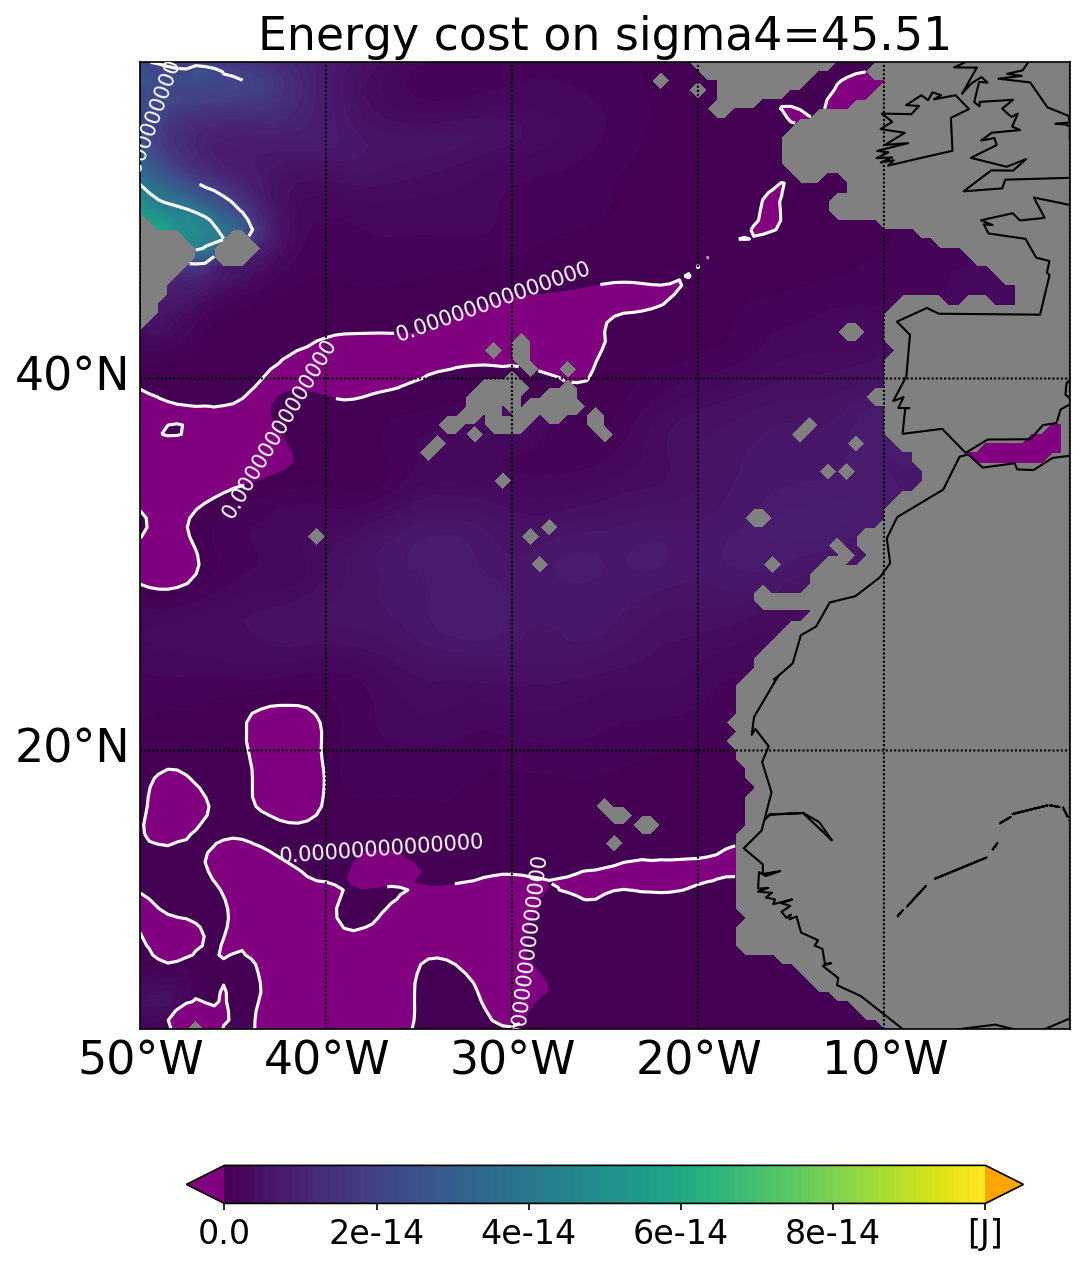
\includegraphics[width=\textwidth]{plots/energy/atlantic_energy/Map2dcyl_energy_on_sigma4_4551e-2_reg310Eto360E05Nto57N_1990to1998av_WOCE.png}
         \caption{$\frac{\Delta E}{d^2}$ on $\sigma_4 = 45.51$, Atlantic}
         \label{fig:subplot_atlantic_energy_sigma_4}
     \end{subfigure}
     \hfill
     \begin{subfigure}[b]{0.4\textwidth}
         
         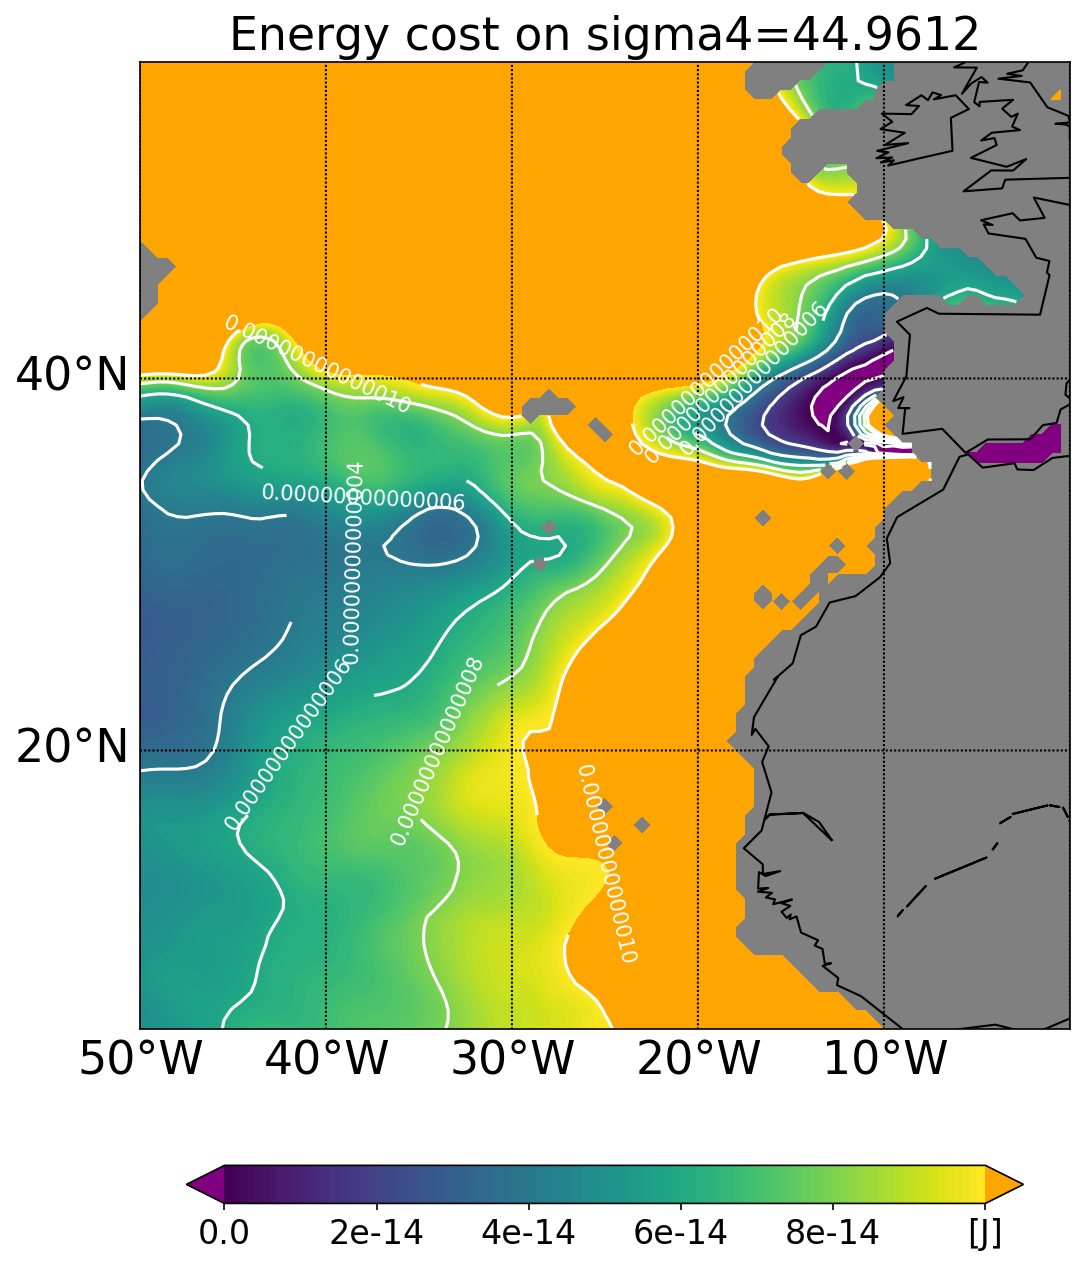
\includegraphics[width=\textwidth]{plots/energy/gibraltar_energy/Map2dcyl_energy_on_sigma4_4496e-2_reg310Eto360E05Nto57N_1990to1998av_WOCE.png}
         \caption{$\frac{\Delta E}{d^2}$ on $\sigma_4 = 44.9612$, Gibraltar}
         \label{fig:subplot_gibraltar_energy_sigma_4}
     \end{subfigure}
     \hfill
      \begin{subfigure}[b]{0.4\textwidth}
         
         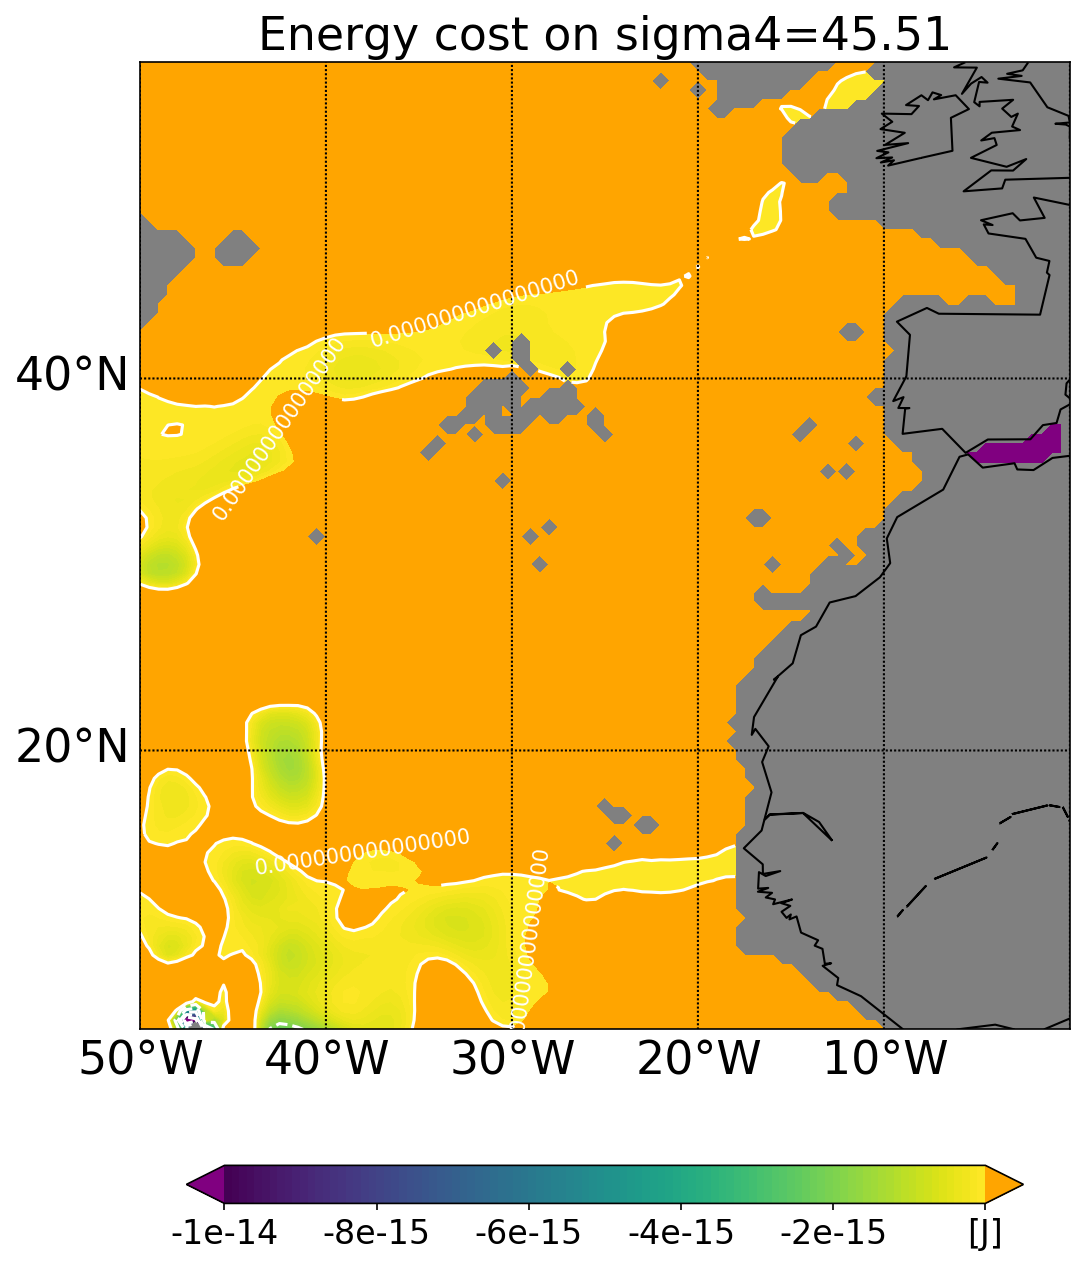
\includegraphics[width=\textwidth]{plots/energy/atlantic_energy/Map2dcyl_neg_energy_on_sigma4_4551e-2_reg310Eto360E05Nto57N_1990to1998av_WOCE.png}
         \caption{$\frac{\Delta E}{d^2}$ on $\sigma_4 = 45.51$, Atlantic}
         \label{fig:subplot_atlantic_neg_energy_sigma_4}
     \end{subfigure}
     \hfill
     \begin{subfigure}[b]{0.4\textwidth}
         
         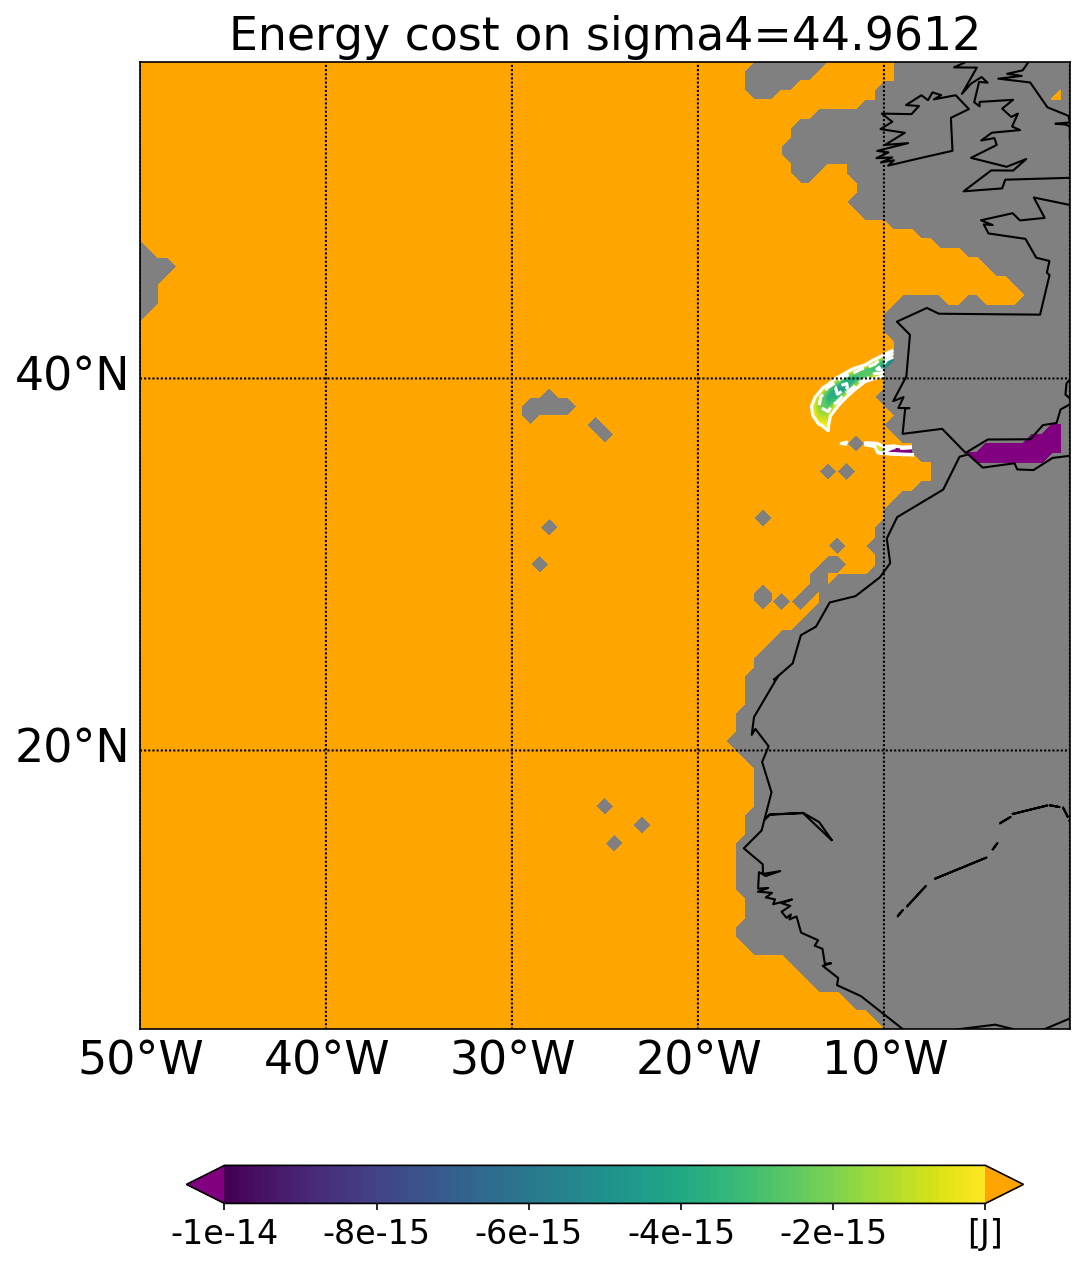
\includegraphics[width=\textwidth]{plots/energy/gibraltar_energy/Map2dcyl_neg_energy_on_sigma4_4496e-2_reg310Eto360E05Nto57N_1990to1998av_WOCE.png}
         \caption{$\frac{\Delta E}{d^2}$ on $\sigma_4 = 44.9612$, Gibraltar}
         \label{fig:subplot_gibraltar_neg_energy_sigma_4}
     \end{subfigure}
     
    \caption{The normalised energy cost, $\frac{\Delta E}{d^2}$, calculated on the the neutral surfaces $\sigma_4 = 45.51$ for the Atlantic region and  $\sigma_4 = 44.9612$ for the Gibraltar region (see section \ref{subsubsection:spreadmethodgibraltarstraight}). Figures (a) and (b) show positive energy cost, figures (c) and (d) show negative energy cost}
    \label{fig:energy_sigma_4}
    
\end{figure}

While these results seem to suggest that the energy cost on the neutral surface is not necessarily zero and that it is possible to have a negative energy cost, the plots are quite messy and this could be for the following two reasons:

Firstly, the \citet{WOCE2002} dataset treats pressure as an alternative to depth coordinates. That is to say it has the same profile for every longitude/latitude point. It is also rounded to integer values. In order to get accurate values for the energy cost it is necessary to have precise pressure data so in order to say with certainty that our results are valid they should be repeated with pressure values that are more specific. These could be found by integrating the density values given in the dataset over the depth, as we have assumed that the ocean is hydrostatic.

Secondly, two parcel energetics are still an approximation to the full dynamics of the energy in a system. Two parcel energetics were used in this work as they are much simpler than the full set. However, a clearer picture may require using the full dynamics. 